\documentclass{article}
\usepackage[utf8]{inputenc}
\usepackage[left=3cm,right=3cm,top=3cm,bottom=3cm,includeheadfoot]{geometry}
\usepackage{ngerman}
\usepackage{xcolor}
\usepackage{float}
\usepackage{listings}
\lstset{
  basicstyle=\ttfamily,
  columns=fullflexible,
  frame=single,
  breaklines=true,
  postbreak=\mbox{\textcolor{red}{$\hookrightarrow$}\space},
}
\usepackage{natbib}
\usepackage{graphicx}
\usepackage{hyperref}
\lstset{basicstyle=\ttfamily,
  showstringspaces=false,
  %commentstyle=\color{red},
  %keywordstyle=\color{blue}
}

%%% Kopf- und Fußzeile
\usepackage{scrpage2}
\pagestyle{scrheadings}
\clearscrheadfoot
\ofoot{\pagemark}

\title{Installation von ROS unter Windows und Visualisierung des Manutec r2 Roboters}
\author{1. Version: Brian Collins, Thomas Loran, Felix Langer}

\date{Februar 2018}

\begin{document}
%%% Titelseite
\maketitle
\thispagestyle{empty}


\begin{figure}[H]
\centering

\includegraphics[scale=1]{Bilder/Logo.png}
\caption{Logo}
\label{fig:Logo}
\end{figure}

\begin{figure}[H]
\centering

\includegraphics[scale=0.35]{Bilder/ROS.png}
\caption{ROS}
\label{fig:ROS}
\end{figure}

\newpage
%%% Inhaltsverzeichnis
\tableofcontents
\thispagestyle{empty}
\newpage

\setcounter{page}{1}
\section{Einleitung}

\subsection{Ziel}
Das Ziel des Projekts ist es die Bewegung des Manutec r2 mit dem Robot Operating System zu visualisieren. Dieser wird mit einer SPS-Software (CODESYS) gesteuert. CODESYS und ROS sollen über das TCP/IP-Protokoll miteinander kommunizieren. 

\subsection{Problemstellung}
Die Problematik liegt in der Kommunikation zwischen ROS und CODESYS, da ROS ausschließlich auf Linux und CODESYS ausschließlich auf Windows läuft. Beide Programme sollen auf dem selben Rechner laufen. Demnach muss eines der beiden Betriebssysteme ein Subsystem des jeweilig anderen Betriebssystems sein.

\subsection{Problemlösung}
Für die Lösung dieses Problems gibt es zwei Varianten. Die erste Variante basiert darauf, das Linux-Betriebssystem in einer virtuellen Maschine unter Windows zu betreiben. Die zweite Variante, die in diesem Projekt verwendet wird, verwendet ein Windows Subsystem für Linux. In der folgenden Dokumentation wird erklärt, wie man dieses Subsystem sowie ROS installiert.
\section{Installation des Linux Subsystems unter Windows}
\subsection{Installation von Xming}
Xming ist eine windowsseitige Software zur Bereitstellung eines X-Servers.\\
...\\
Xming ist eine freie Software und kann unter folgender URL gedownloaded werden:\\
\url{https://sourceforge.net/projects/xming/}

\begin{figure}[h!]
\centering

\includegraphics[scale=0.7]{Bilder/Xming.PNG}
\caption{Download Xming}
\label{fig:Xming}
\end{figure}\\ \\Nach dem Download der Installationsanweisung folgen und das Programm Xming starten, nicht den Xming Launcher! Xming läuft nun im Hintergrund und kann jederzeit über die Taskleiste beendet werden.

\subsection{Freischaltung des Features}
Um das Windows Subsystem für Linux zu aktivieren, muss zuerst das Feature aktiviert werden. Dafür öffnet man die Windows PowerShell als Administrator und führt folgenden Befehl aus:
\begin{lstlisting}[language=bash]
Enable-WindowsOptionalFeature -Online -FeatureName Microsoft-Windows-Subsystem-Linux
\end{lstlisting}

Zum Schluss noch mit \textit{Y} bestätigen um den Rechner neu zu starten.

\begin{figure}[H]
\centering
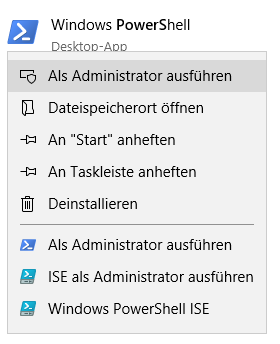
\includegraphics[scale=0.8]{Bilder/PowerShell.PNG}
\caption{Windows PowerShell}
\label{fig:PowerShell}
\end{figure}

\begin{figure}[H]
\centering
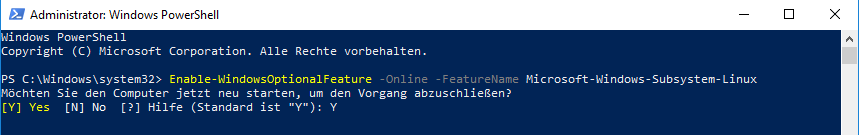
\includegraphics[scale=0.5]{Bilder/Befehl.PNG}
\caption{Befehl}
\label{fig:Befehl}
\end{figure}



\subsection{Installation von Ubuntu}
Die passende Installation von Ubuntu für das Subsystem findet man im Microsoft Store.

\begin{figure}[H]
\centering

\includegraphics[scale=1]{Bilder/Store.PNG}
\caption{Microsoft Store}
\label{fig:Store}
\end{figure}

Dort sucht man nach Ubuntu und installiert es.

\begin{figure}[H]
\centering
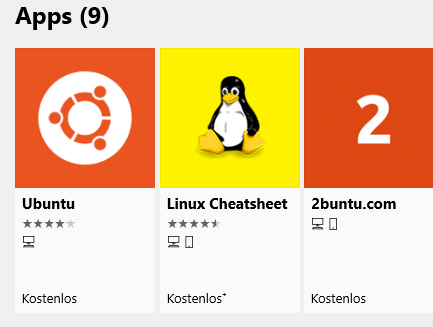
\includegraphics[scale=0.8]{Bilder/Ubuntu.PNG}
\caption{Ubuntu}
\label{fig:Ubuntu}
\end{figure}

\subsection{Einrichten von Ubuntu}
\subsubsection{Anlegen eines Benutzers}
Nach erfolgreicher Installation wird man nun aufgefordert, einen neuen Benutzer anzulegen.

\subsubsection{Testen der grafischen Oberfläche}
Bevor man Xming als X-Server verwenden kann, muss das Display bei jedem Start aktiviert werden. Damit dieser Vorgang bei jedem Start des Subsystems ausgeführt wird, muss folgendes in die Datei \textit{.bashrc} geschrieben werden:\\
Zuerst muss in das Root-Verzeichnis gewechselt werden:
\begin{lstlisting}[language=bash]
cd
\end{lstlisting}

Jetzt kann die Datei mit dem Nano Texteditor geöffnet werden:
\begin{lstlisting}[language=bash]
nano .bashrc
\end{lstlisting}

Folgender Befehl wird jetzt ganz unten eingefügt:
\begin{lstlisting}[language=bash]
export DISPLAY=:0
\end{lstlisting}
Zum Speicher \textit{STRG+O} drücken und zum beenden \textit{STRG+X}.

Danach werden die benötigten Pakete installiert:
\begin{lstlisting}[language=bash]
sudo apt-get install x11-apps
\end{lstlisting}
Jetzt kann die grafische Ausgabe getestet werden:

\begin{lstlisting}[language=bash]
xclock
\end{lstlisting}
Es sollte nun ein Fenster geöffnet werden, auf dem eine Uhr abgebildet ist. Ist dies der Fall, funktioniert der X-Server.
\begin{figure}[H]
\centering
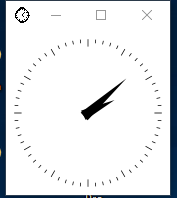
\includegraphics[scale=0.8]{Bilder/Clock.PNG}
\caption{XClock}
\label{fig:XClock}
\end{figure}

\subsubsection{Installation eines grafischen Terminals}
Da für die Verwendung von ROS mehrere Terminals benötigt werden, wird ein grafisches Terminal installiert, das über eine Tabverwaltung verfügt. Mit dem folgendem Befehl lässt sich das Terminal Sakura installieren.
\begin{lstlisting}[language=bash]
sudo apt-get install sakura
\end{lstlisting}
Zum ausführen des Terminals, folgenden Befehl in die Windows Bash eintippen:
\begin{lstlisting}[language=bash]
sakura
\end{lstlisting}
Jetzt öffnet sich in einem seperaten Fenster ein weiteres Terminal das ab sofort das Hauptterminal ist. Nun ist es möglich mit der rechten Maustaste weitere Tabs zu öffnen.



\subsection{Starten von Ubuntu}
Nach der Installation landet man automatisch in der Ubuntu-Umgebung. Möchte man aber nach einem Neustart Ubuntu ausführen, muss folgender Befehl in die Windows Eingabeaufforderung(CMD) eingegeben werden:
\begin{lstlisting}[language=bash]
bash
\end{lstlisting}

\begin{figure}[H]
\centering
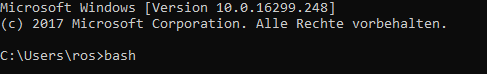
\includegraphics[scale=1.0]{Bilder/Bash.PNG}
\caption{Bash}
\label{fig:Bash}
\end{figure}

\subsection{Beenden von Ubuntu}
Zum beenden von Ubuntu müssen alle grafischen Terminals geschlossen werden, bis auf die Windows Bash. In der Windows Bash kommt man nun mit folgendem Befehl wieder auf das Windows Betriebssystem und beendet damit Ubuntu:
\begin{lstlisting}[language=bash]
exit
\end{lstlisting}

\section{ROS}

\subsection{Was ist ROS?}
Das Robot Operating System oder kurz ROS, ist ein Meta-Betriebssystem welches sich über das eigentliche Betriebssystem legt. Das ROS bedient arbeitet, ähnlich wie das MQTT-Protokoll, mit dem Public/Subscribe-Prinzip. Es funktioniert ausschließlich auf Linux und versteht die Syntax von C++ und Phyton. 
Der Vorteil des ROS ist, dass man eine Vielzahl an Packages hat, welche man ohne großen Aufwand in sein Projekt einbinden kann. Des Weiteren muss man über keinerlei Wissen über das Package verfügen um damit arbeiten zu können.

\subsection{Installation von ROS}
Die folgende Installationsanleitung von ROS bezieht sich auf ROS Kinetic und Xenial (Ubuntu 16.04).\\
Zuerst muss man die ROS Pakete und Schlüssel hinzufügen:
\begin{lstlisting}[language=bash]
sudo sh -c 'echo "deb http://packages.ros.org/ros/ubuntu $(lsb_release -sc) main" > /etc/apt/sources.list.d/ros-latest.list'
\end{lstlisting}

\begin{lstlisting}[language=bash]
sudo apt-key adv --keyserver hkp://ha.pool.sks-keyservers.net:80 --recv-key 421C365BD9FF1F717815A3895523BAEEB01FA116
\end{lstlisting}
Vor der Installation müssen alle Pakete auf dem aktuellsten Stand sein:
\begin{lstlisting}[language=bash]
sudo apt-get update
\end{lstlisting}
Jetzt kann mit der ROS Installation begonnen werden:
\begin{lstlisting}[language=bash]
sudo apt-get install ros-kinetic-desktop-full
\end{lstlisting}
Dieser Vorgang kann je nach verbauter Hardware etwas Zeit in Anspruch nehmen.\\
Bevor man nun ROS starten kann, müssen noch einige Befehle ausgeführt werden:
\begin{lstlisting}[language=bash]
sudo rosdep init
\end{lstlisting}

\begin{lstlisting}[language=bash]
rosdep update
\end{lstlisting}

\begin{lstlisting}[language=bash]
echo "source /opt/ros/kinetic/setup.bash" >> ~/.bashrc
\end{lstlisting}

\begin{lstlisting}[language=bash]
source ~/.bashrc
\end{lstlisting}

\begin{lstlisting}[language=bash]
source /opt/ros/kinetic/setup.bash
\end{lstlisting}

\subsection{Einrichten des Workspaces}
Damit man Nodes in ROS ausführen kann, muss zuerst das Arbeitsverzeichnis erstellt werden. Hierfür müssen folgende Befehler in der Linux-Console ausgeführt werden:
\begin{lstlisting}[language=bash]
mkdir -p ~/catkin_ws/src
\end{lstlisting}

\begin{lstlisting}[language=bash]
cd ~/catkin_ws/src
\end{lstlisting}

\begin{lstlisting}[language=bash]
catkin_init_workspace
\end{lstlisting}

\begin{lstlisting}[language=bash]
cd ~/catkin_ws/
\end{lstlisting}

\begin{lstlisting}[language=bash]
source devel/setup.bash
\end{lstlisting}

\begin{lstlisting}[language=bash]
catkin_make
\end{lstlisting}

\subsection{Testen der Installation}
Mit der Simulation TurtleSim kann man ganz einfach testen, ob die Installation geklappt hat. Mit folgenden Befehlen lässt sich die Simulation starten (jeder Befehl = neuer Tab!):

\begin{lstlisting}[language=bash]
roscore
\end{lstlisting}

\begin{lstlisting}[language=bash]
rosmake turtlesim
\end{lstlisting}

\begin{lstlisting}[language=bash]
rosrun turtlesim turtlesim_node
\end{lstlisting}

\begin{lstlisting}[language=bash]
rosrun turtlesim turtle_teleop_key
\end{lstlisting}

Es kann passieren, dass der TurtleSim nicht auf die Tastertureingabe reagiert, dann muss das aktive Fenster der Node \textit{turtle\_teleop\_key} sein.



\section{Visualisierung des Manutec r2 unter ROS}

\subsection{Installieren der Nodes}
Um das Projekt einzubinden müssen die folgenden Kommandos der Reihe nach ausgeführt werden. \\ \\
Zu erst geht man in den richtigen Workspace, welcher der Catkin Workspace ist. 

\begin{lstlisting}[language=bash]
cd ~/catkin_ws/src/
\end{lstlisting}
Anschließend wird das Projekt aus Github kopiert und mit folgendem Befehl eingefügt (Tipp: Man kann den Link auch einfach aus der Dokumentation kopieren)
\begin{lstlisting}[language=bash]
git clone https://github.com/informatik-mannheim/virtual-robot-ros.git
\end{lstlisting}
Um das Projekt zu kompilieren muss man den unten ausgeführten Befehl ausführen. Dies muss man auch bei jeder Änderung machen um das Projekt zu aktualisieren.
\begin{lstlisting}[language=bash]
cd ~/catkin_ws/
\end{lstlisting}

\begin{lstlisting}[language=bash]
catkin_make
\end{lstlisting}

\subsection{Starten der Nodes}
Um das Meta-Betriebssystem ROS zu starten wird folgender Befehl benötigt
\begin{lstlisting}[language=bash]
roscore
\end{lstlisting}
Starten des TCP-Server Nodes:
\begin{lstlisting}[language=bash]
rosnode ...
\end{lstlisting}
Starten der Manutec r2 Simulation:
\begin{lstlisting}[language=bash]
roslaunch ...
\end{lstlisting}



\subsection{Simulation des Manutec r2 Roboters}
Um das Projekt zu simulieren wird die Codesys Datei ausgeführt. Diese startet automatisch auch das ROS und die Launch-Datei, die die Bewegungen des Roboters simuliert. 

\subsection{Beenden der Nodes}
Zum beenden der Nodes, einfach mit \textit{STRG+C} den aktuellen Node schließen.




\newpage

%%% Abbildungsverzeichnis
\listoffigures
\thispagestyle{empty}

\end{document}